


\documentclass[a4paper,11pt]{article}
 \pdfoutput=1 % if your are submitting a pdflatex (i.e. if you have
             % images in pdf, png or jpg format)
\usepackage{jinstpub} 


% for details on the use of the package, please
                     % see the JINST-author-manual



\title{The Readout system of the CBM Projectile Spectator Detector at FAIR}


\author[a,c,1]{D. Finogeev,\note{Corresponding author.}}
\author[a,b]{F. Guber,}
\author[a]{N. Karpushkin,}



\affiliation[a]{Institute for Nuclear Research RAS, Moscow, Russia,}
\affiliation[b]{Moscow Institute of Physics and Technology, Dolgoprudny, Moscow Region, Russia}
\affiliation[c]{National Research Nuclear University MEPhI, Moscow, Russia}
\affiliation[d]{ Joint Institute for Nuclear Research, Dubna, Russia}


% e-mail addresses: only for the forresponding author
\emailAdd{dmitry.finogeev@cern.ch}




\abstract{Abstract: The Projectile Spectator Detector (PSD),  a sampling lead/scintillator forward hadron calorimeter with transverse and longitudinal segmentation and with MPPCs photodetectors, will be used at the Compressed Baryonic Matter (CBM) experiment at FAIR to measure the centrality and orientation of the reaction plane in nucleus-nucleus collisions. After amplification in the FEE, signals from the MPPCs are readout with LMT9011 ADCs with 14 bit digitization and up to 125 Msps rate which has been developed for the ECAL of the PANDA experiment at FAIR.  The Kintex 7 FPGA is used for signal processing and data collection. The trigger-less readout is based on the GBT-FPGA. Clock source switching from onboard generator to the RX clock transmitted via GBT has been implemented to integrate the ADC board into the CBM DAQ system. One PSD module has been integrated into the mCBM experiment at the SIS18 facility of GSI/FAIR joining the FAIR Phase-0 program. Details of the PSD readout electronics and first results of the data processing and transmission within the common, synchronized mCBM data transport taken during the data campaign in November/December 2019 are shown. }



\keywords{Hadron calorimeters, trigger-less readout, GBT readout}

\collaboration[c]{on behalf of CBM collaboration}



\begin{document}
\maketitle
\flushbottom

\section{The CBM experiment at FAIR}
\label{sec:intro}
The future Compressed Baryonic Matter (CBM) experiment at the Facility for Antiproton and Ion Research (FAIR) is aimed to explore the Quantum Chromodynamics (QCD) phase diagram in the region of high baryon densities. The CBM will operate in the beam energy range of 2 - 11 AGeV and beam interaction rates up to 10 MHz. The CBM experiment will use a free-streaming data acquisition system (DAQ), which requires a coordinated time stamping of data in all sub-systems. This coordination includes a time-stamping against related clocks (common base), a synchronization procedure (deterministic time offsets) and the delivery of data containers of identical size during the data taking. The forward hadron compensating lead/scintillator calorimeter - the Projectile Spectator Detector (PSD), with transverse and longitudinal segmentation and with the micropixel photodetectors light readout will be used in the CBM experiment to measure the event centrality and the reaction plane orientation in heavy-ion collisions. The mCBM setup at SIS18 is a prototype and demonstrator for CBM and the first implementation of a combined readout with CBM subsystems of different front-end electronics types.


\section{The Projectile spectator detector design}
The PSD is assembled from 46 individual modules, each forming a lead-scintillation sandwich. Schematic view and photo of a single PSD module are represented in figure~\ref{fig:1}. Light readout from each scintillator plate is provided by WLS-fibers embedded in grooves in the scintillator plates. Six consecutive scintillator tiles form a section and are connected to a single photodetector at the end of the module. The longitudinal segmentation of the modules into 10 sections ensures the uniformity of light collection along the modules. Hamamatsu MPPCs S12572-010P with active area 3$\times$3 $mm^2$ are used as photodetectors for each section of module. 
Thus, the entire detector accounts for 460 signal readout channels.


\\////////////////////////FEE??///////////////\\

Each photodetector is provided with a reference voltage of about 70 volts, as well as individual automatic correction of the reference voltage depending on the external temperature. The temperature sensor, as well as the LED for the possibility of photoelectronic calibration of photodiodes, are placed on the FEE panel. The monitoring and data collection from all FEEs are carried out by means of the slow control system.

\\/////////////////to Makhnev/////////////////\\

\begin{figure}[htbp]
\centering 
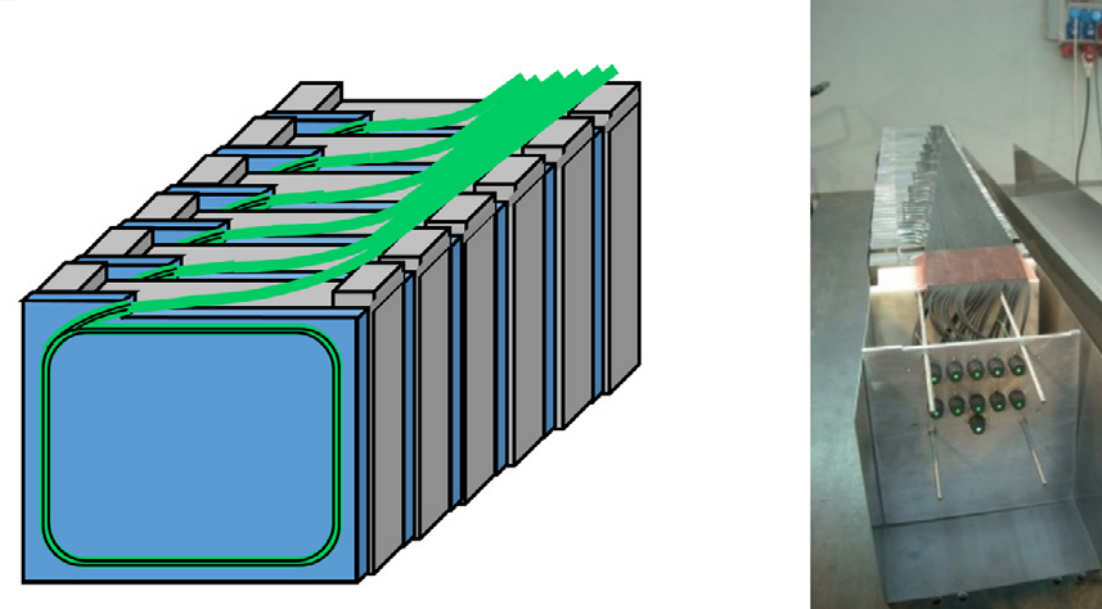
\includegraphics[width=.45\textwidth]{PSD_module.png}
\caption{\label{fig:1} Schematic view of the sampling lead/scintillator module, (left). Photo of the PSD module (right)}
\end{figure}



\section{PSD readout concept}
Signals from MPPCs are collected by the ADC addon board represented in figure~\ref{fig:2} (left). Addon board provides a single-ended interface based on single-ended to differential converters AD8138 IC that allow to provide adjustable input offset. The PSD readout is accomplished by the ADC board designed for the ECAL detector of PANDA experiment \cite{1} (see figure~\ref{fig:1}, right). The 64-channel board based on ADC LTM9011 with digitization rate up to 125Msps and 14-bit digitization resolution. ADC used now in 80 Msps digitization mode, the setup will be upgraded up to 120 Msps in 2020. 
Digitized samples of 64 analog signals are sent to 2 FPGAs Kintex 7 using 128 LVDS links. Each FPGA process data from 32 channels. For current tests simple signals waveform analyzing algorithm is used triggered by threshold crossing and provide charge of signal in fixed gate. Advanced signal processing algorithm is developing based on prony-fitting method that allow increase charge resolution and pile-up recognizing. 
To meet requirement of experiment DAQ, GBT FPGA transceiver was integrated into firmware. GBT allow to transmit data, slow control and clock. Expected data rate is 1MHz per channel that constrains 100bit/hit for GBT data rate 3.2 Gbit/s. 
LMK0460 jitter cleaner used for production ADC and MGTREF clocks. After reset 100MHz clock from on-board generator TD-100 used as master clock. After GBT RX synchronization established, source switched to external clock sourced from GBT RX. The clock switching scheme allow to maintain common DAQ clock domain. Measuring hit time in trigger-less readout occurs relative to time counting named timeslice synchronous for all experiment readout.

\begin{figure}[htbp]
\centering % \begin{center}/\end{center} takes some additional vertical space
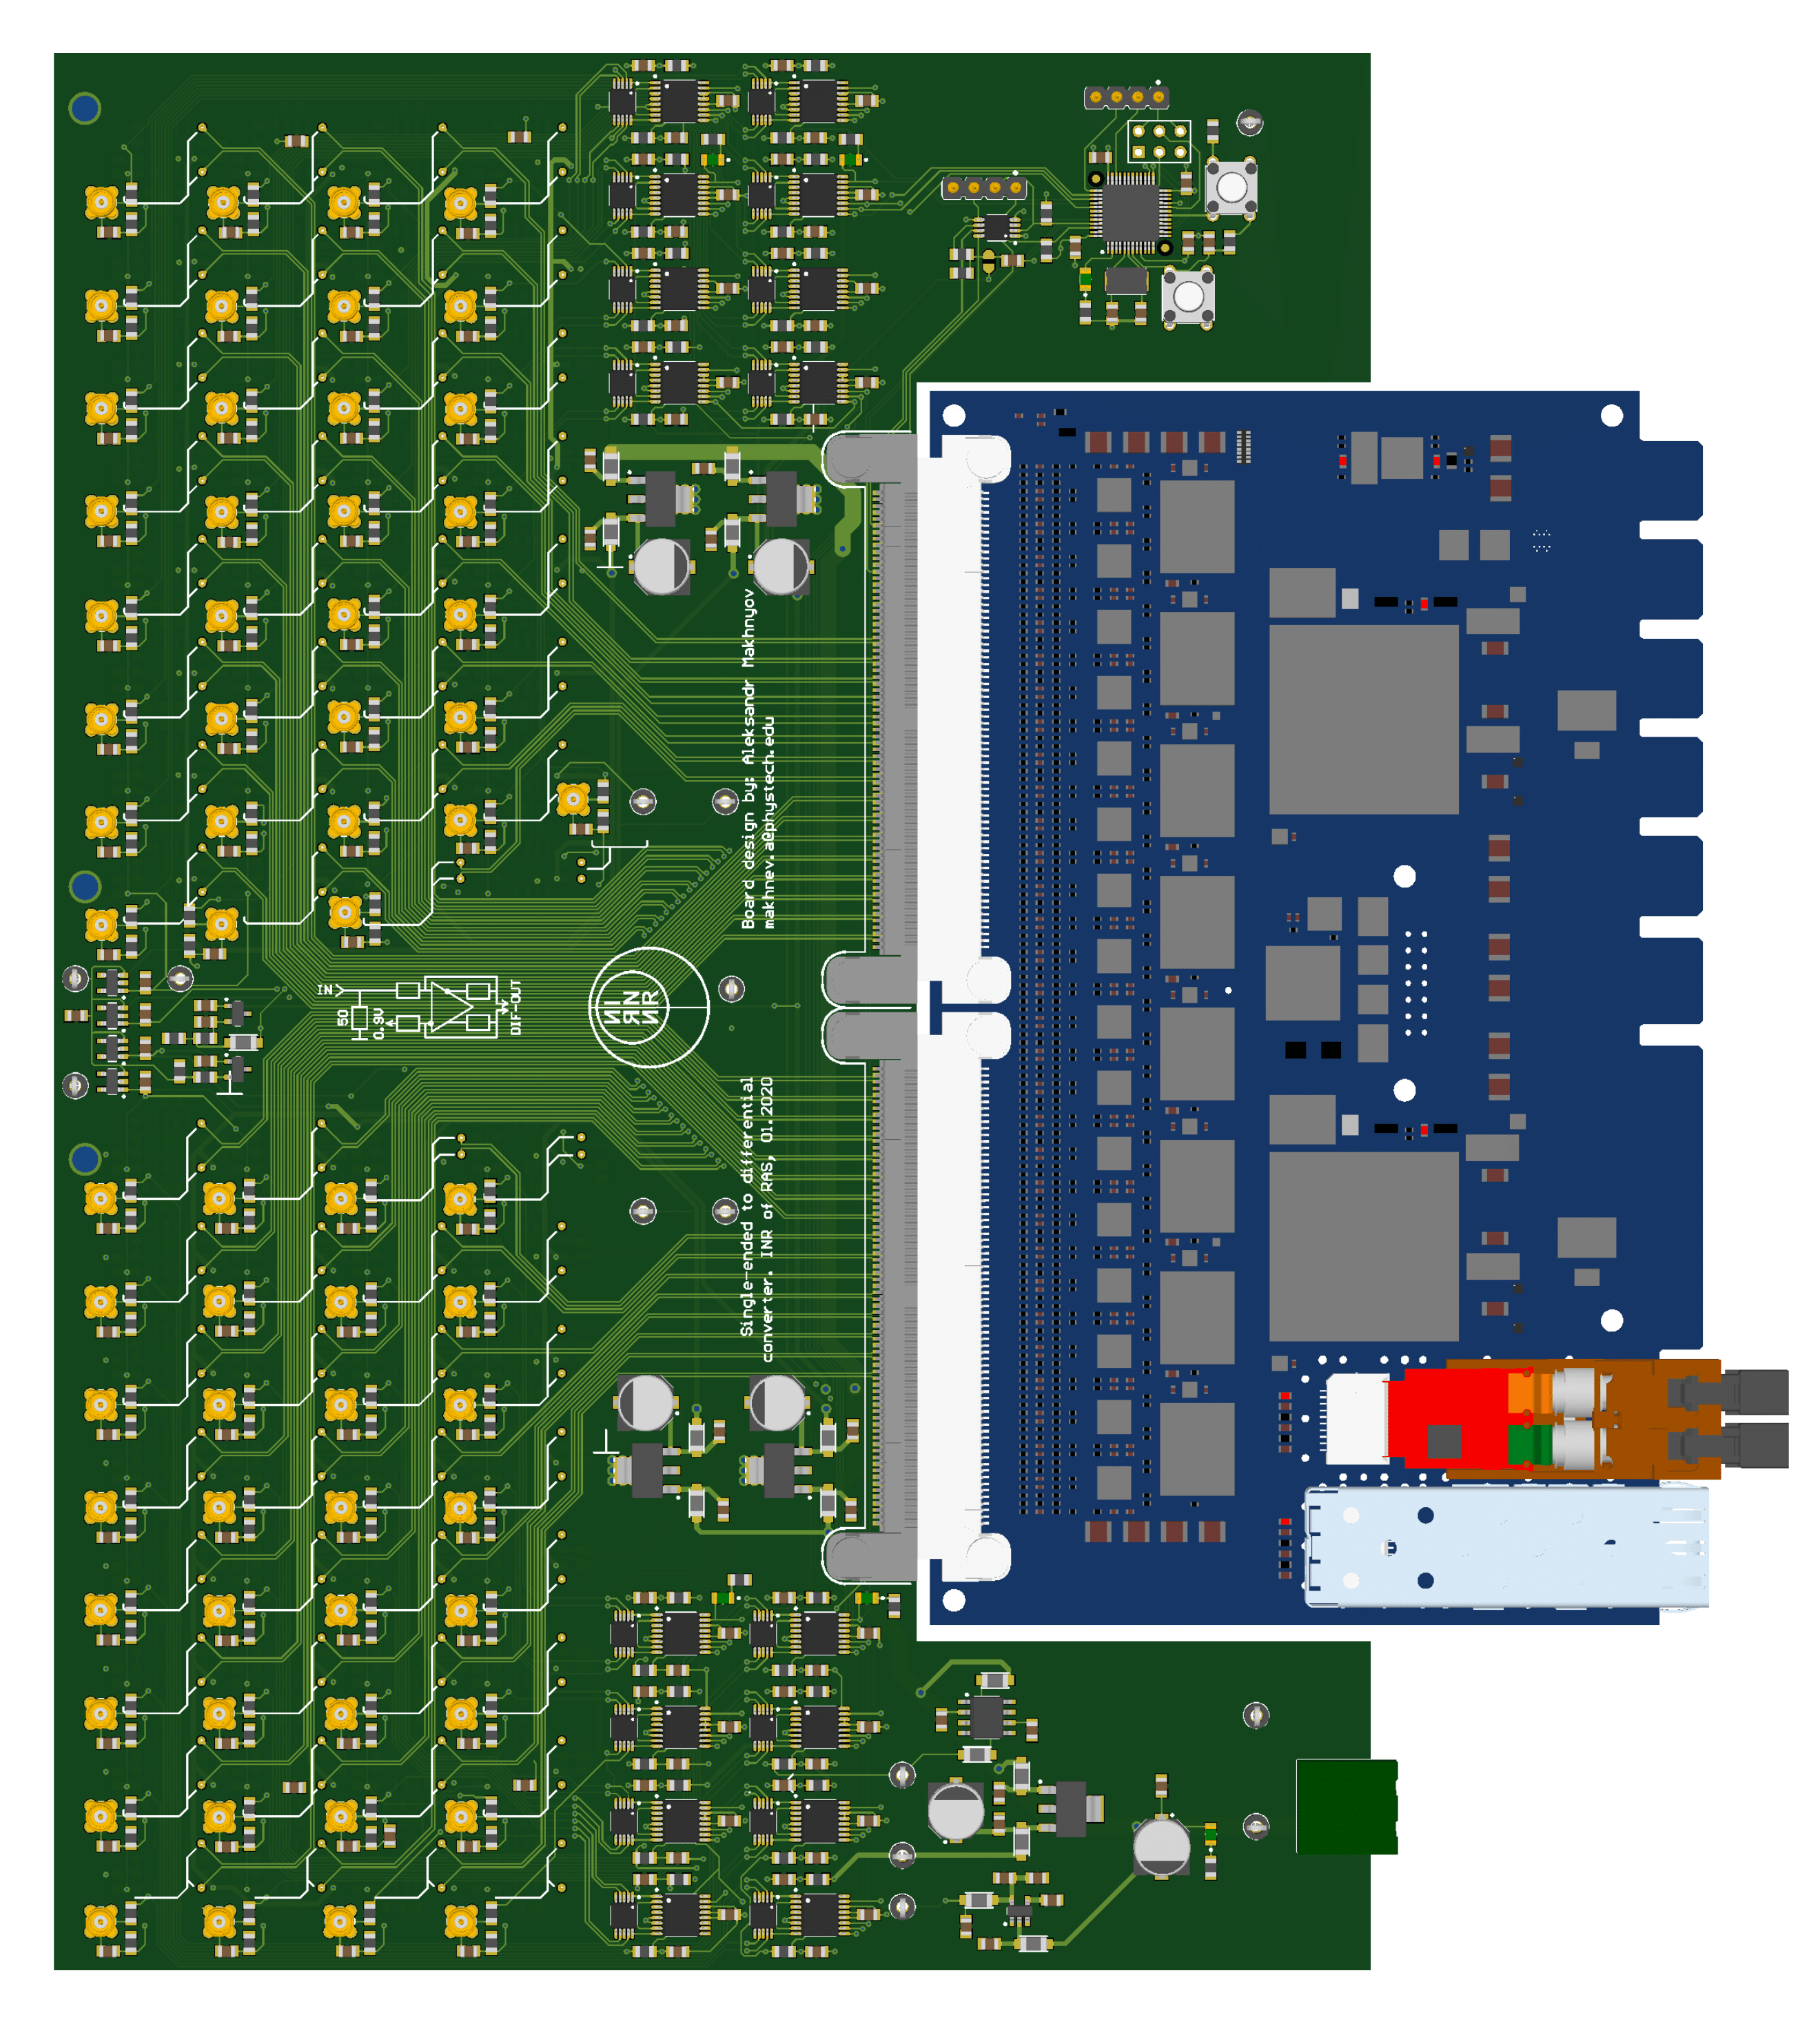
\includegraphics[width=.5\textwidth]{ADC_addon.png}
\qquad
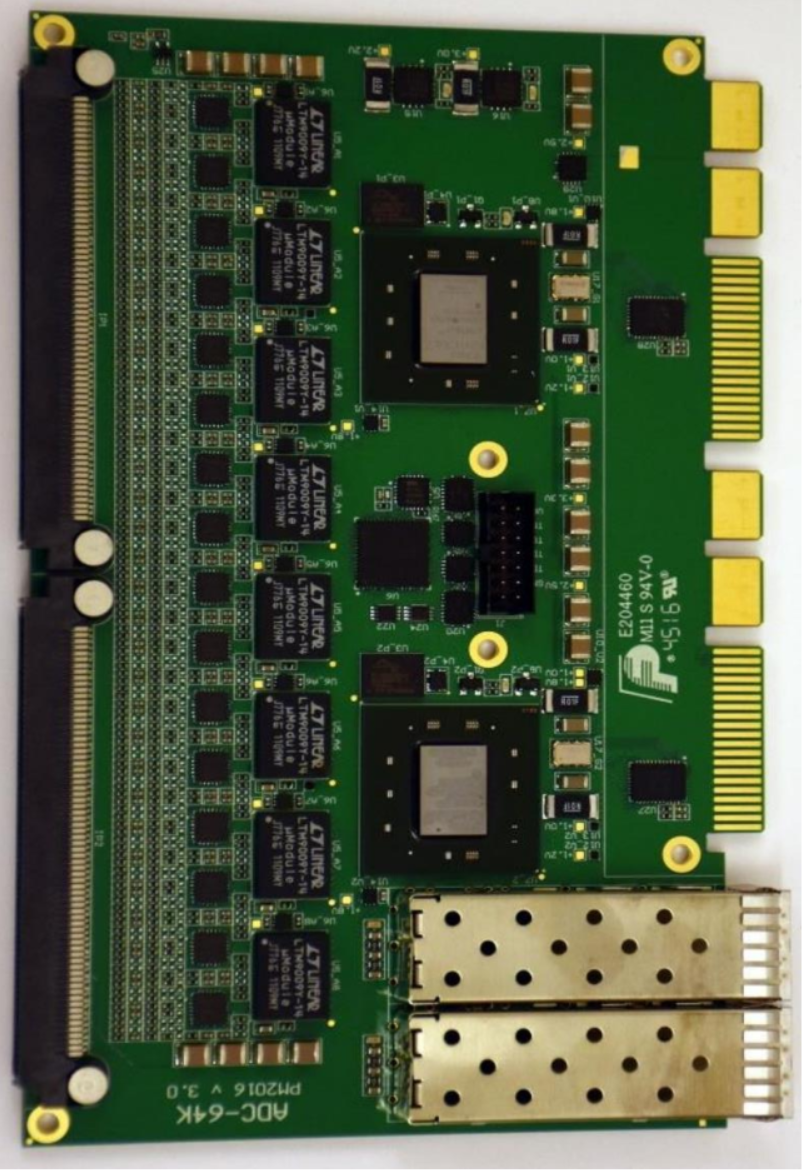
\includegraphics[width=.2\textwidth]{ADC_board.png}

\caption{\label{fig:2} 64-channel ADC board with 2 FPGA Kintex 7 (right). 64-channel ADC board addon  based on single-ended to differential converters (left) }
\end{figure}


\acknowledgments
This work was supported by the Russian Foundation of Basic Research (RFBR) Grant No. 1



\begin{thebibliography}{99}



\bibitem{1}
F.~Guber \textit{et al.} [NA61/SHINE, CBM and BM@N],
\emph{Transverse and longitudinal segmented forward hadron calorimeters with SiPMs light readout for future fixed target heavy ion experiments},
Nucl.\ Instrum.\ Meth.\ A \textbf{958} (2020), 162728
doi:10.1016/j.nima.2019.162728


\bibitem{2}
Serneguet Sorli, Á. (2015). \emph{A multichannel digitizer for the PANDA experiment.} http://hdl.handle.net/10251/56722.



\end{thebibliography}
\end{document}

